\documentclass[a4paper,10pt]{article}
\usepackage[utf8x]{inputenc}
\usepackage{verbatim}
\usepackage{graphicx}
\usepackage{float}

%opening
\title{}
\author{}

\begin{document}

\maketitle

\section{myps.sh}

\subsection{Code}
\verbatiminput{myps.sh}

\subsection{Screenshot}
\begin{figure}[H]
 \centering
 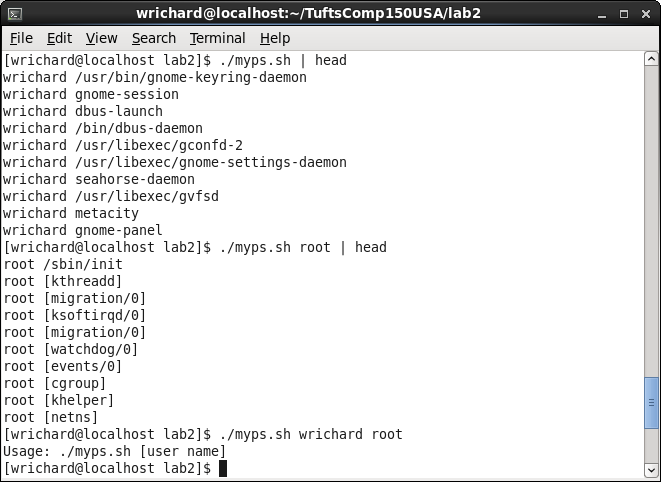
\includegraphics[width=\linewidth]{./myps.png}
 % myps.png: 0x0 pixel, 0dpi, nanxnan cm, bb=
 \caption{myps output}
 \label{fig:myps}
\end{figure}

\section{calc.sh}

\subsection{Code}
\verbatiminput{calc.sh}

\subsection{Screenshot}
\begin{figure}[H]
 \centering
 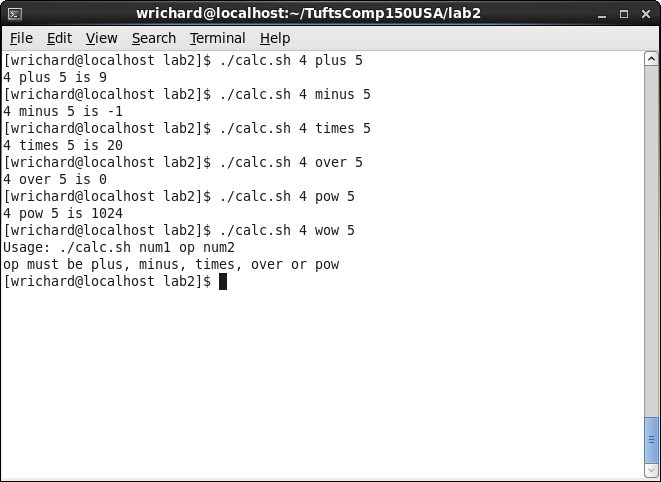
\includegraphics[width=\linewidth]{./calc.png}
 % myps.png: 0x0 pixel, 0dpi, nanxnan cm, bb=
 \caption{calc output}
 \label{fig:myps}
\end{figure}

\section{sum.sh}

\subsection{Code}
\verbatiminput{sum.sh}

\subsection{Screenshot}
\begin{figure}[H]
 \centering
 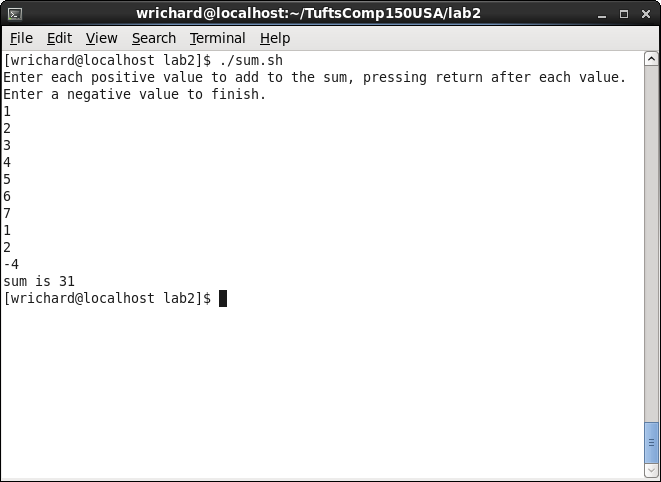
\includegraphics[width=\linewidth]{./sum.png}
 % myps.png: 0x0 pixel, 0dpi, nanxnan cm, bb=
 \caption{sum output}
 \label{fig:myps}
\end{figure}

\section{print\_lines.sh}

\subsection{Code}
\verbatiminput{print_lines.sh}

\subsection{Screenshot}
\begin{figure}[H]
 \centering
 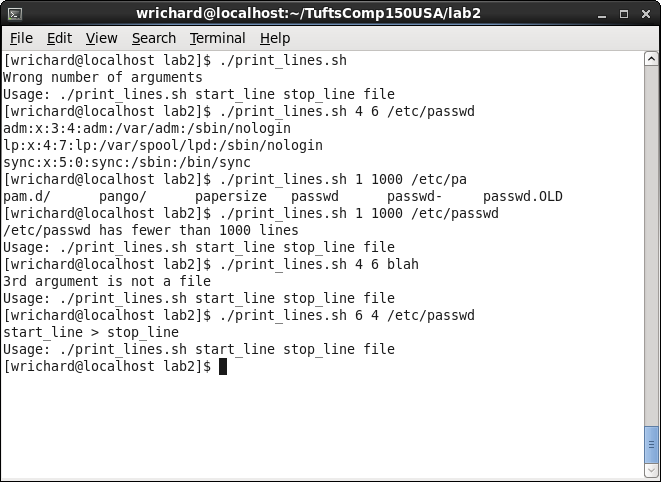
\includegraphics[width=\linewidth]{./print_lines.png}
 % myps.png: 0x0 pixel, 0dpi, nanxnan cm, bb=
 \caption{print\_lines output}
 \label{fig:myps}
\end{figure}

\end{document}
